% Options for packages loaded elsewhere
\PassOptionsToPackage{unicode}{hyperref}
\PassOptionsToPackage{hyphens}{url}
%
\documentclass[
]{article}
\usepackage{lmodern}
\usepackage{amssymb,amsmath}
\usepackage{ifxetex,ifluatex}
\ifnum 0\ifxetex 1\fi\ifluatex 1\fi=0 % if pdftex
  \usepackage[T1]{fontenc}
  \usepackage[utf8]{inputenc}
  \usepackage{textcomp} % provide euro and other symbols
\else % if luatex or xetex
  \usepackage{unicode-math}
  \defaultfontfeatures{Scale=MatchLowercase}
  \defaultfontfeatures[\rmfamily]{Ligatures=TeX,Scale=1}
\fi
% Use upquote if available, for straight quotes in verbatim environments
\IfFileExists{upquote.sty}{\usepackage{upquote}}{}
\IfFileExists{microtype.sty}{% use microtype if available
  \usepackage[]{microtype}
  \UseMicrotypeSet[protrusion]{basicmath} % disable protrusion for tt fonts
}{}
\makeatletter
\@ifundefined{KOMAClassName}{% if non-KOMA class
  \IfFileExists{parskip.sty}{%
    \usepackage{parskip}
  }{% else
    \setlength{\parindent}{0pt}
    \setlength{\parskip}{6pt plus 2pt minus 1pt}}
}{% if KOMA class
  \KOMAoptions{parskip=half}}
\makeatother
\usepackage{xcolor}
\IfFileExists{xurl.sty}{\usepackage{xurl}}{} % add URL line breaks if available
\IfFileExists{bookmark.sty}{\usepackage{bookmark}}{\usepackage{hyperref}}
\hypersetup{
  hidelinks,
  pdfcreator={LaTeX via pandoc}}
\urlstyle{same} % disable monospaced font for URLs
\usepackage{longtable,booktabs}
% Correct order of tables after \paragraph or \subparagraph
\usepackage{etoolbox}
\makeatletter
\patchcmd\longtable{\par}{\if@noskipsec\mbox{}\fi\par}{}{}
\makeatother
% Allow footnotes in longtable head/foot
\IfFileExists{footnotehyper.sty}{\usepackage{footnotehyper}}{\usepackage{footnote}}
\makesavenoteenv{longtable}
\usepackage{graphicx}
\makeatletter
\def\maxwidth{\ifdim\Gin@nat@width>\linewidth\linewidth\else\Gin@nat@width\fi}
\def\maxheight{\ifdim\Gin@nat@height>\textheight\textheight\else\Gin@nat@height\fi}
\makeatother
% Scale images if necessary, so that they will not overflow the page
% margins by default, and it is still possible to overwrite the defaults
% using explicit options in \includegraphics[width, height, ...]{}
\setkeys{Gin}{width=\maxwidth,height=\maxheight,keepaspectratio}
% Set default figure placement to htbp
\makeatletter
\def\fps@figure{htbp}
\makeatother
\setlength{\emergencystretch}{3em} % prevent overfull lines
\providecommand{\tightlist}{%
  \setlength{\itemsep}{0pt}\setlength{\parskip}{0pt}}
\setcounter{secnumdepth}{-\maxdimen} % remove section numbering

\author{}
\date{}

\begin{document}

\hypertarget{dlxsim}{%
\section{Dlxsim}\label{dlxsim}}

Dlxsim {[}DLX-Package{]} is an instruction accurate simulator for DLX
assembly code. In this laboratory, we will use a modified version of
dlxsim, which is changed in such a way, that it is behaving like the
ASIP Meister specific implementation of the Brownie STD 32 Processor,
which will be created and used in the later steps of the laboratory. In
the first subchapter, some basic ideas about the Brownie architecture
and the Brownie instruction set will be introduced. Afterwards the basic
usage of dlxsim will be explained. In the last subchapter, it is shown
how dlxsim can be extended to support new assembly instructions, which
will be added to the Brownie processor with ASIP Meister.

\hypertarget{brownie-std-32-architecture}{%
\subsection{Brownie STD 32
Architecture}\label{brownie-std-32-architecture}}

Brownie STD 32 (browstd32.pdb) is a RISC-type pipeline processor
architecture. The Brownie architecture is designed for an easy and fast
\textbf{pipeline processor}. It is a \textbf{Load-/Store-architecture},
which means that there are dedicated commands for accessing the memory
and that all the other commands only work on registers, but not on
memory addresses. As an implication, the Brownie architecture has a
\textbf{big uniform register file} that consists of 32 registers with 32
bits each, where some registers are special registers like the register
r0 has a special meaning, as it is hard wired to zero. The pipeline
stages for the Brownie processor are the following:

\begin{enumerate}
\def\labelenumi{\arabic{enumi}.}
\item
  Instruction Fetch (\textbf{IF}): This phase reads the command on which
  the program counter (PC) points from the instruction memory into the
  instruction register (IR) and increases the PC.
\item
  Instruction Decode (\textbf{ID}): Here the instruction format is
  determined and the respectively needed parameters are prepared; e.g.
  reading a register from the register file or sign extending an
  immediate value.
\item
  Execute (\textbf{EXE}): The specific operation is executed in this
  phase for the parameters, which have been prepared in the preceding
  stage.
\item
  Memory Access and Write Back (\textbf{WB}): If the command is a memory
  access, then the access will be executed in this phase. Every
  non-memory access command will pass this stage without any activity.
  Finally, the result that has been computed or loaded will be written
  back to the register file.

  The memory architecture of Brownie STD is Harvard. Both of the
  instruction length and the data length are 32 bit. Addressing can be
  performed in byte. Brownie has 32 integer general-purpose registers
  and a 4-stage pipeline structure, each stage of which is named IF, ID,
  EXE and WB. Full forwarding to the pipeline makes the operation
  results of all the instructions immediately usable. Brownie STD
  executes delayed load for load type instruction, and the number of
  delayed slot is one. Brownie STD does not have a delayed branch slot
  (does not execute delayed branch). Brownie STD does not have a
  floating-unit operation. A floating-point execution instruction can be
  added as a custom instruction. Basic architecture parameters are shown
  in the following table.

  In \protect\hyperlink{Fig32}{Figure 3-2}, an example for some
  overlapping commands in a 5-stage pipeline (DLX processor) is shown.
  In the first command, the values from the registers \emph{r2} and
  \emph{r3} are added and the result is stored in register \emph{r1}.
  The write back to \emph{r1} is done in clock cycle 4, so it cannot be
  read earlier than in clock cycle 5. The last command of the shown
  pipeline example is using \emph{r1} as input and it is scheduled in
  such a way, that it is reading \emph{r1} in clock cycle 5, so that it
  is using the latest value that has just been written back by the first
  command. \emph{The example shows, that three successive NOPs are
  enough to resolve a data dependency.} The Brownie processor is using a
  \textbf{data forwarding} technique to resolve such data dependencies
  without the in-between NOPs, and ASIP Meister does support full
  forwarding i.e. data and branch forwarding is available in this
  version of ASIPmeister. Therefore, for ASIP Meister generated
  processors, the NOPs are not needed to resolve the data dependencies
  (as shown in Chapter~3.2.1 you can configure dlxsim to behave in both
  ways, i.e. with or without data forwarding).
\end{enumerate}

\begin{longtable}[]{@{}ll@{}}
\toprule
\textbf{Parameters} & \textbf{Architecture}\tabularnewline
\midrule
\endhead
Basic architecture & RISC\tabularnewline
Memory architecture & Harvard\tabularnewline
Instruction length & 32\tabularnewline
Data length & 32\tabularnewline
Addressing & Byte address\tabularnewline
The number of general-purpose registers & 32\tabularnewline
The number of pipeline stages & 4\tabularnewline
The number of delayed branch slot & 0\tabularnewline
Floating-point unit & N/A\tabularnewline
Forwarding & full forwarding\tabularnewline
Alignment & 1-byte, 2-byte and 4-byte\tabularnewline
Endian-ness & Big Endian\tabularnewline
Interrupts & Reset, Internal, External\tabularnewline
\bottomrule
\end{longtable}

Figure 3‑1: Brownie STD 32 Architecture Parameters

The \textbf{instruction set} of the BROWSTD32 architecture is separated
into four \textbf{instruction classes} (arithmetic for integer,
arithmetic for float, load/store and branch), which are implemented in
different \textbf{instruction formats}, as shown in
\protect\hyperlink{Fig33}{Figure 3-3}. The arithmetic instructions use
either an instruction format for three registers or an instruction
format for two registers and an immediate value. The load/store
instructions always use the format with two registers and one immediate,
where the effective address is computed as the sum of one register (as
base address) and the immediate value. The other register is used either
as value to store in memory or as register where to place the loaded
value. The branch instructions are divided into conditional branches and
unconditional jumps. The jumps use an instruction format with a 26-bit
immediate value as a PC-relative jump-target. The \emph{jump register}
instructions instead use the I-Format to declare in which register the
absolute jump target is placed. The second register and the immediate
value are not used by these instructions. The conditional branches need
a field for a register that contains the condition, so they use the
I-Format as well. They use the 16-bit immediate as PC relative jump
target. The second available register is not used.
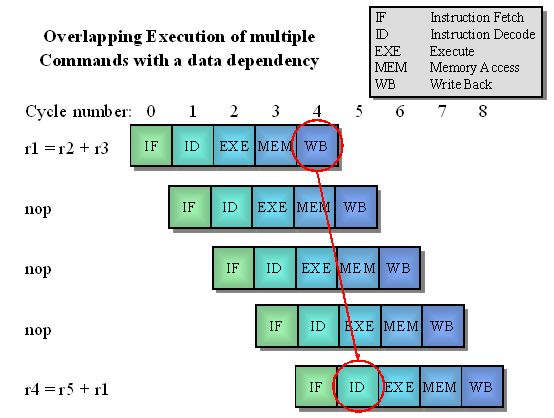
\includegraphics[width=6.09196in,height=3.97917in]{3-2.png}
Figure 3‑2\protect\hypertarget{Fig32}{}{}: BROWSTD32 Pipeline Example
with a Data Dependency

For many assembly-commands, there are special versions for dealing with
unsigned values and for using immediate values as second input
parameters. These versions have an attached ``i'' for ``immediate''
and/or an attached ``u'' for ``unsigned'' as suffix (e.g. addui). A
summary of all assembly instructions that are available in the ASIP
Meister specific implementation of the BROWSTD32 processor that is used
in the laboratory (i.e. browstd32) is shown in Figure 3‑4:. For a more
detailed description of the assembly-commands have a look into
{[}Sailer96{]}.

Finally, some specialties in the architecture need to be mentioned:

\begin{itemize}
\item
  \textbf{Delay slots:} Without forwarding, an instruction, that is
  placed right after an unconditional jump or a conditional branch
  instruction is always executed. In fact, there are two instructions,
  that enter the pipeline, but only the first one is executed, the
  second one will not be allowed to write the computed result back to
  the register file. But, in Brownie this is handled automatically using
  full-forwarding.
\item
  \textbf{Multicycle operations:} The operations mult, div and mod in
  their different versions are multicycle operations. That means, that
  these operations will not stay for one cycle in the execute phase, but
  for multiple cycles. The pipeline is stalled until the instructions
  finished their work in the execute stage.
\item
  \textbf{Stalling:} The communication to the data memory is controlled
  by Request/Acknowledge-Signals to deal with memories of different
  speed. The corresponding assembly instructions might stay for multiple
  cycles in the memory stages, until the memory access is finished.
\end{itemize}

%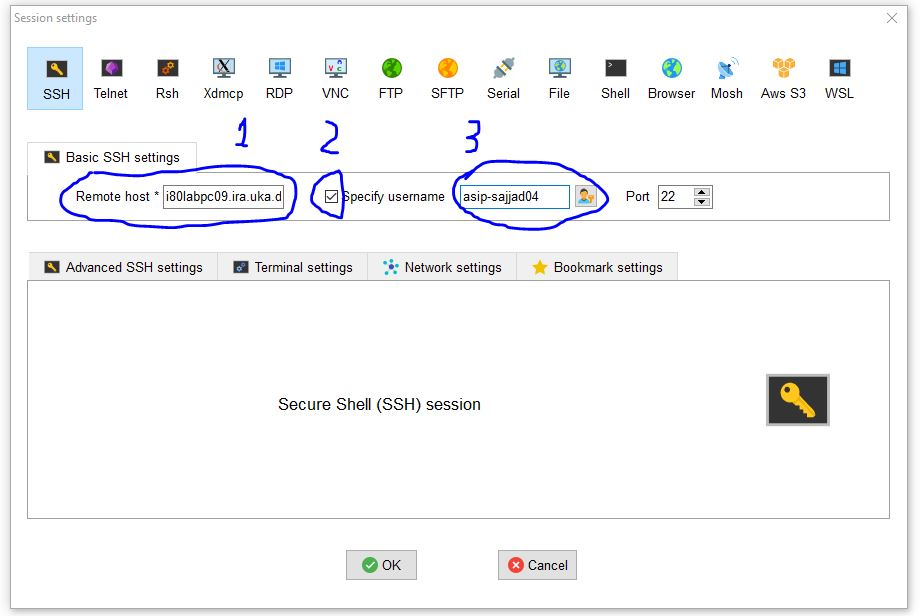
\includegraphics[width=6.29167in,height=7.90833in]{media/image2.emf}
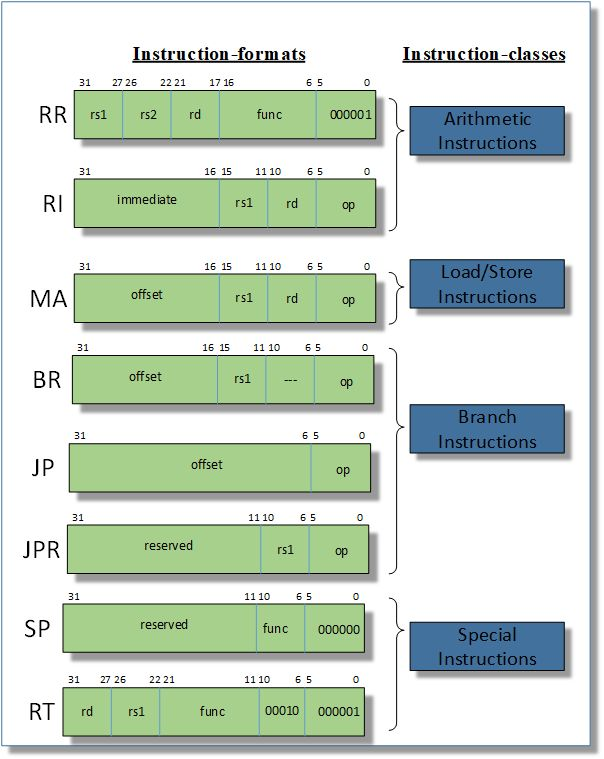
\includegraphics[width=6.09196in,height=3.97917in]{3-3.png}
\protect\hypertarget{Fig33}{}{}Figure 3‑3: Instruction Formats and
Classes of the BROWSTD32 Architecture

\begin{itemize}
\item
  \textbf{Special Registers:} Some registers in the general-purpose
  register file usually handle some special cases. However, contrary to
  the hard-wired zero-register \emph{r0}, any register, as long it is
  done consistent in the assembly file, can handle these other special
  cases. These special cases are the stack pointer (GPR\emph{1}), the
  frame pointer (GPR4) and the link register (\emph{GPR3}), which is
  then used as return address. For more details, please look into the
  Page-9 of Brownie Reference Manual {[}{]}.
\item
  \textbf{Instructions:} for more details of the instruction and their
  syntax refer to Page-44 {[}RM{]}
\end{itemize}

\begin{longtable}[]{@{}llll@{}}
\toprule
\endhead
\textbf{Instruction} & \textbf{Description} & \textbf{Instruction} &
\textbf{Description}\tabularnewline
\emph{ADD, ADDI} & Add; Syntax: \emph{add rd rs0 rs1;} \emph{rs1} can
alternatively be the immediate & \emph{SUB, SUBI} &
Subtract\tabularnewline
\emph{MUL} & Multiply & \emph{DIV, DIVU} & Divide\tabularnewline
\emph{MOD, MODU} & Modulo & \emph{AND, ANDI} & And\tabularnewline
\emph{OR, ORI} & Or & \emph{XOR, XORI} & Xor\tabularnewline
\emph{LLS, LLSI} & Shift left logical & \emph{LRS, LRSI} & Shift right
logical\tabularnewline
\emph{ARS, ARSI} & Shift right arithmetic & \emph{ELT, ELTU} & Set
``less than''; Syntax: \emph{slt rd rs0 rs1;} Compare \emph{rs0} and
\emph{rs1} and set \emph{rd} to 1 if and only if rs0 is ``less than''
rs1\tabularnewline
\emph{LSOI} & Left shift \& OR immediate value & \emph{NAND,NOR} & Nand
, NOR operation\tabularnewline
\emph{ENEQ} & Set ``not equal'' & \emph{EEQ} & Set
``equal''\tabularnewline
\emph{LB} & Load Byte & \emph{LH} & Load High\tabularnewline
\emph{LW} & Load Word; Syntax: \emph{load rd, imm(rs);} the effective
address is computed by adding the immediate to \emph{rs} & \emph{SB} &
Store Byte; Syntax: \emph{store imm(rd), rs;} the effective address is
computed by adding the immediate to \emph{rd}\tabularnewline
\emph{SH} & Store High & \emph{SW} & Store Word\tabularnewline
\begin{minipage}[t]{0.22\columnwidth}\raggedright
\emph{BRZ}\strut
\end{minipage} & \begin{minipage}[t]{0.22\columnwidth}\raggedright
Branch if ``equal zero''

Syntax: branch rs, imm; the branch target is a PC-relative address,
given by the immediate\strut
\end{minipage} & \begin{minipage}[t]{0.22\columnwidth}\raggedright
\emph{BRNZ}\strut
\end{minipage} & \begin{minipage}[t]{0.22\columnwidth}\raggedright
Branch if ``not equal zero''\strut
\end{minipage}\tabularnewline
\emph{JP (JPR)} & Jump (Register); Syntax\emph{: j imm (jr rs);} The
jump target is a PC-relative (absolute) address, given by the immediate
(register) & \emph{JPL (JPLR)} & Jump and link (Register); Similar to
\emph{j/jr}, but also writes the address from the following command to
the link register; used for subroutine calls\tabularnewline
\emph{NOP} & & \emph{RETI} & Return Interrupt\tabularnewline
\emph{EXBW} & 8-bit to 32-bit sign extension & \emph{EXHW} & 16-bit to
32-bit sign extension\tabularnewline
\bottomrule
\end{longtable}

Figure 3‑4: Summary of All Assembly Instructions in the \emph{browstd32}
Processor

\hypertarget{extending-dlxsim}{%
\subsection{Extending dlxsim}\label{extending-dlxsim}}

\hypertarget{startup-parameters-for-dlxsim}{%
\subsubsection{Startup Parameters for
dlxsim}\label{startup-parameters-for-dlxsim}}

Some parameters can be adapted when starting dlxsim. All mentioned
parameters in Figure 3‑5: do not allow blanks between a parameter, e.g.
``\emph{-pf0}'' instead of ``\emph{-pf~0}''.

\begin{longtable}[]{@{}ll@{}}
\toprule
\endhead
\textbf{Option} & \textbf{Description}\tabularnewline
-f\emph{filename} & This parameter will load an assembly file after
initialization. This parameter is equivalent to the instruction
``\emph{load \{filename\}}'' in Figure 3‑7:.\tabularnewline
-sf\emph{filename} & This parameter loads a script file that can contain
any command that you can type within dlxsim. These commands are then
executed one after the other. For simulation automation, you can forward
the output of dlxsim to a file (\emph{make dlxsim {[}\ldots{]}
\textgreater{} foo.txt}) and then extract the needed information out of
this file (\emph{grep ``Total cycles'' foo.txt}).\tabularnewline
\begin{minipage}[t]{0.47\columnwidth}\raggedright
-dbb\#

(Debug Base Blocks)\strut
\end{minipage} & \begin{minipage}[t]{0.47\columnwidth}\raggedright
This option only has an effect, if the later mentioned option
``\emph{Debug Assembly}'' is enabled too. If both options are activated,
then a register snapshot will automatically be printed at every base
block start. This snapshot only includes registers, for which the value
has changed since the last snapshot. By default, this option is turned
off to avoid the enormous amount of output. To turn it on you have to
enter \emph{``-dbb1}''.\strut
\end{minipage}\tabularnewline
\begin{minipage}[t]{0.47\columnwidth}\raggedright
-da\#

(Debug Assembly)\strut
\end{minipage} & \begin{minipage}[t]{0.47\columnwidth}\raggedright
This option helps you debugging the simulated assembly code. A debugging
output is printed for all load/store and jump/branch instructions,
including in which cycle the message was printed and from which address
it was triggered. By default, this option is turned on. To turn it off
you have to enter \emph{``-da0}''.\strut
\end{minipage}\tabularnewline
\begin{minipage}[t]{0.47\columnwidth}\raggedright
-cdd\#

(Check Data Dependency)\strut
\end{minipage} & \begin{minipage}[t]{0.47\columnwidth}\raggedright
With this option, you enable a warning message that appears when an
unresolved data dependency is found in the executed assembly code. This
means you will get a warning if for example, \emph{r5} is read in cycle
10, but an earlier command has made a write access to \emph{r5}, that
cannot be read back before cycle 12. Therefore, you would read the `old'
value. By default, this option is turned on. To turn it off you have to
enter ``\emph{-cdd0}''.\strut
\end{minipage}\tabularnewline
\begin{minipage}[t]{0.47\columnwidth}\raggedright
-wsdo\#

(Warn Specific Dependency Once)\strut
\end{minipage} & \begin{minipage}[t]{0.47\columnwidth}\raggedright
This option belongs to the before mentioned option Check Data
Dependency. If there is an unresolved data dependency in a loop, then
the warning message would usually be printed for every time the loop is
executed. With this option defined, the warning will only be printed the
first time the unresolved data dependency is noticed. By default, this
option is turned on. To turn it off you have to enter
\emph{``-wsdo0}''.\strut
\end{minipage}\tabularnewline
\begin{minipage}[t]{0.47\columnwidth}\raggedright
-pf\#

(Pipeline Forwarding)\strut
\end{minipage} & \begin{minipage}[t]{0.47\columnwidth}\raggedright
With this option, you can configure, whether you have a ``Full
Forwarding'' (1) or not (0). In case of forwarding, your operands are
forwarded to next stages and no branch delay slot is required. But, even
in case of forwarding, you still require a delay slot (nop) for
loar/store.\strut
\end{minipage}\tabularnewline
\begin{minipage}[t]{0.47\columnwidth}\raggedright
-ms\#

(Memory Size)\strut
\end{minipage} & \begin{minipage}[t]{0.47\columnwidth}\raggedright
The size of the memory that is available within dlxsim. It is the common
memory for instructions and data.\strut
\end{minipage}\tabularnewline
-lf\emph{filename} & With this parameter, all print instructions for the
LCD (as shown in Chapter~8.3.1) are written to a file instead of the
screen.\tabularnewline
-uf\emph{filename} & With this parameter, all print instructions for the
UART (as shown in Chapter~8.3.2) are written to a file instead of the
screen.\tabularnewline
-af\emph{filename} & With this parameter, all outputs to the AudioOut
IP-Core (as shown in Chapter~8.3.2) are written to a file instead of the
screen.\tabularnewline
\bottomrule
\end{longtable}

Figure 3‑5: Summary of Helpful dlxsim Starting Parameters

Legend: \emph{cursive}: replace with appropriate option, \#: replace
with a number

\hypertarget{how-to-add-a-new-instruction}{%
\subsubsection{How to Add a New
Instruction}\label{how-to-add-a-new-instruction}}

The following list shows you the needed steps to add a new instruction
for a given instruction-format. The given line numbers are rounded and
might change during time, as the source code is partially under
development. Every needed part of the source code is marked with a
comment that includes the string ``\emph{ASIP NEW\_INSTRUCTIONS}''.

\begin{enumerate}
\def\labelenumi{\arabic{enumi}.}
\item
  \emph{dlx.h}:222 Add a new define for \textbf{OP\_\{CommandName\}}
  with a unique number.
\item
  \emph{sim.c}:227 Add the \textbf{name} for your assembly-command into
  the \textbf{operationNames}-array. The position of the name in this
  array has to correspond with the defined number in \emph{dlx.h} from
  the preceding step.
\item
  \emph{asm.c}:338 Add a new entry with your instruction name,
  instruction format and opcode into the \emph{\textbf{opcodes}}-table
  ``OpcodeInfo opcodes{[}{]}''. The \textbf{instruction name} has to be
  the same like in the previous step and completely written in
  lower-case! The already available \textbf{instruction formats} are
  shown in Figure 3‑6:. There are two different possibilities for the
  \textbf{opcode}. Either you use the only ``opcode'' or you use
  ``opcode'' and ``func'' field collectively. The unused bits always
  stay 0 in the opcode field. These two possibilities differ in how
  dlxsim is internally handling the instruction. This will become
  clearer in the following step. Have a look at the following step to
  find free opcodes. The following values in the opcode table are
  usually not that important and might be filled out by copy-and-paste
  from a similar instruction. Only the flags are important if you use
  instructions with immediate values as parameter. The flags are
  explained in \emph{asm.c}.
\item
  \emph{sim.c}:362 This step depends on your choice of the preceding
  step. You have used either the ``opcode'' or the ``opcode'' plus
  ``func'' field. If you have only ``opcode'' field, then you have to
  modify the \emph{\textbf{opTable}} in \emph{sim.c} otherwise in case
  of ``opcode and func'' field, then you have to modify the
  \emph{\textbf{specialTable}}. In both cases you replace the table
  entry at the position that corresponds to the chosen 6-bit opcode with
  your own \emph{\textbf{OP\_\{CommandName\}}}. So if you have chosen
  the opcode value 5, then you replace the 5\textsuperscript{th} entry
  (start counting with 0) in the array with your own command.
\item
  \emph{sim.c}:2197 Implement a new \textbf{case} for the big
  ``\emph{\textbf{switch (wordPtropcode)}}''-statement for your command.
  A good start is a copy-and-paste from a similar instruction. There are
  2 different variables for the parameters. For example, there is a
  ``\emph{\textbf{wordPtrrs1}}'' and a ``\emph{\textbf{rs1}}''. In
  ``\emph{\textbf{wordPtrrs1}}'' the number of the first source register
  is stored, while in ``\emph{\textbf{rs1}}'' the value of this source
  register is stored. At the beginning of an implementation of one
  specific ``\emph{\textbf{case}}'' some macros like
  ``\emph{\textbf{LoadRegisterS1}}'' are called. These macros take care,
  that ``\emph{\textbf{rs1}}'' is initialized with the current value of
  the register with the number ``\emph{\textbf{wordPtrrs1}}''.
\item
  Compiling: To test your modified version of dlxsim you have to
  re-compile it. Simply type ``make'' in the dlxsim directory.
\end{enumerate}

When the error ``\emph{Unknown Opcode}'' occurs while loading the
assembly file, then the corresponding instructions was not accepted. If
you are sure, that it is not a typing error in the assembly file
(register names, immediate values, \ldots) then have a look into points
1 -- 4.

\hypertarget{how-to-add-a-new-instruction-format}{%
\subsubsection{How to Add a New
Instruction-Format}\label{how-to-add-a-new-instruction-format}}

Adding a new instruction format is much more difficult than adding a new
instruction for a given format. To add a new format you have to take
care about how the parameters for your new format are to be stored in a
32-bit instruction word and how they are extracted out of it. Every
needed part of the source code is marked with a comment that includes
the string ``ASIP NEW\_FORMAT''.

\begin{enumerate}
\def\labelenumi{\arabic{enumi}.}
\item
  \emph{asm.c:}140 Define a unique number for your instruction-format
\item
  \emph{asm.c:}150 Add the \emph{min} and \emph{max} numbers of
  arguments, that your instruction format accepts in the arrays
  ``\textbf{minArgs}'' and ``\textbf{maxArgs}''. Use the position in the
  array, that corresponds to the defined number in the previous step.
\item
  \emph{asm.c:}765 Implement how the parameters will be stored in the
  32-bit instruction word within the ``\textbf{switch
  (insPtr-\textgreater class)}''-statement.
\item
  \emph{asm.c}:1080 Implement what will be written if the instruction is
  disassembled in the ``\textbf{switch
  (opPtr-\textgreater class)}''-statement.
\item
  \emph{sim.c:}2215 In the method ``\textbf{compile}'' you have to
  implement how the 32-bit instruction word will be expanded.
\item
  Compiling To test your modified version of dlxsim you have to
  re-compile it. Simply type ``make'' in the dlxsim directory.
\end{enumerate}

\begin{longtable}[]{@{}ll@{}}
\toprule
\endhead
\textbf{Instruction Format} & \textbf{Parameters}\tabularnewline
NO\_ARGS & no operands\tabularnewline
LOAD & (register, address)\tabularnewline
STORE & (address, register)\tabularnewline
LUI & (dest, 16-bit expression)\tabularnewline
ARITH\_2PARAM & (dest, src) OR (dest, 16-bit immediate) OR "dest"
replaced by "dest/src1"\tabularnewline
ARITH\_3PARAM & (dest, src1, sr2c) OR (dest/src1, src2) OR (dest, src1,
16-bit immediate) OR (dest/src1, 16-bit immediate)\tabularnewline
ARITH\_4PARAM & (rd, rs1, rs2, rs3) OR (rd, rs1, rs2, 5-bit
immediate)\tabularnewline
BRANCH\_0\_OP & (label) the source register is implied\tabularnewline
BRANCH\_1\_OP & (src1, label)\tabularnewline
BRANCH\_2\_OP & (src1, src2, label)\tabularnewline
JUMP & (label) OR (src1)\tabularnewline
SRC1 & (src1)\tabularnewline
LABEL & (label)\tabularnewline
MOVE & (dest,src1)\tabularnewline
\bottomrule
\end{longtable}

Figure 3‑6: Summary of Available dlxsim Instruction Formats

\hypertarget{using-dlxsim}{%
\subsection{Using dlxsim}\label{using-dlxsim}}

Dlxsim is distributed as source code, so before using it you have to
compile it. Usually this is done, by just typing ``\emph{make''} in the
``\emph{tcl''} subdirectory and afterwards in the ``\emph{dlxsim''}
directory. Then you can start the program by typing ``dlxsim''. If you
want to use dlxsim for an ASIP Meister Project, then you have to set
``\emph{DLXSIM\_DIR}'' (see \protect\hyperlink{Fig25}{Figure 2-5}) to
the path where dlxsim is located e.g.
"\emph{/home/asip00/epp/dlxsim\_Laboratory}'', and then typing
``\emph{make dlxsim}'' in an application's subdirectory.

Figure 3‑7: shows some typical dlxsim commands. The list is not
exhaustive, but it covers all the usual suspects.

\begin{longtable}[]{@{}ll@{}}
\toprule
\endhead
\textbf{Command} & \textbf{Description}\tabularnewline
load \emph{filename\textsuperscript{+}} & Load a file, parse its
content, and place the translated content to the simulated memory. Every
address that is not mentioned in the file remains it old
value.\tabularnewline
\begin{minipage}[t]{0.47\columnwidth}\raggedright
get \emph{address} \{\emph{options}\}\strut
\end{minipage} & \begin{minipage}[t]{0.47\columnwidth}\raggedright
Examples for ``\emph{address}'' are \emph{r0}\ldots{} \emph{r31},
\emph{pc}, \emph{npc} (next pc), 10 (memory address 10), 0x10 (memory
address 16), \_main (if \_main is a label).

Examples for ``\emph{options}'' are: u (unsigned), d (decimal), x
(hexadecimal, default), B (binary), i (instruction), v (do not read a
value, but print the address itself; as example this can be used to
translate from decimal to binary), s (interpret the upcoming sequence as
0-terminated string). In the options, you can also request to get the
succeeding addresses from the determined base address. As an example,
``\emph{get \_loop 10i}'' would deliver the 10 first commands from the
label \emph{\_loop} interpreted as instruction memory. This also works,
if the address is a register, e.g. ``\emph{get r1 5u}''.\strut
\end{minipage}\tabularnewline
put \emph{address data} & Place some data at the given address. The
address might be a register too, like in the ``\emph{get''}
command.\tabularnewline
step \{\emph{number}\} & Execute the next number of instructions given
by ``\emph{number}'', the default value is 1. The printed assembly
command at the end of ``\emph{step}'' is the next assembly command that
is to be executed.\tabularnewline
go \{\emph{address}\} & Execute the assembly program, until an error
occurs or a trap instruction is executed. It starts executing at
``\emph{address}''. If no ``\emph{address}'' is given, then it continues
executing where it is stopped (e.g. after some single steps). The
default address is 0.\tabularnewline
stats \{\emph{options}\} & Print some statistics about the simulated
assembly program. The \emph{options} are explained in more detail in
Chapter~3.3.1.\tabularnewline
quit exit & Terminates the program\tabularnewline
\begin{minipage}[t]{0.47\columnwidth}\raggedright
stop \{\emph{options}\}\strut
\end{minipage} & \begin{minipage}[t]{0.47\columnwidth}\raggedright
Manages break points:

``\emph{stop at address \{command\}}'': Executes ``\emph{command}''
whenever the given ``\emph{address}'' is touched in any way. The default
``\emph{command}'' is to abort the execution.

``\emph{stop info}'': prints the list of break points.

``\emph{stop delete number\textsuperscript{+}}'': deletes some specific
break points. The numbers are according to the ``\emph{stop info}''
list.\strut
\end{minipage}\tabularnewline
asm ``\emph{command}'' \{\emph{pc}\} & Return the opcode for
``\emph{command}''. If the command needs to know the address where it is
to be stored (e.g. pc-relative jumps), then the current pc can be given.
Default pc is 0.\tabularnewline
\bottomrule
\end{longtable}

Figure 3‑7: Summary of Typical dlxsim Commands

\textbf{Legend}: \emph{cursive}: replace with appropriate option,
\{braces\}: optional, \textsuperscript{+}: one or multiple times

Some more points that have to be mentioned about dlxsim are:

\begin{itemize}
\item
  You can use the cursor buttons to navigate in your command history,
  i.e. in the previously entered commands. The up- and down-arrow-keys
  let you navigate inside the selected command, e.g. to correct typing
  errors.
\item
  When you just enter an empty command in dlxsim (i.e. just press enter
  without having entered a command), then the last executed command will
  be repeated. This is for example useful, when you want to step through
  your code. You just have to execute the step instruction one time
  manually by typing ``\emph{step}'' in the shell and afterwards you can
  repeatedly press enter to execute the next step instructions.
\item
  When you press the Tab key, you will get an auto completion for
  filenames. The offered files are the files in the directory from where
  you started dlxsim. Although this auto completion will support the
  abbreviation ``\emph{\textasciitilde{}}'' for your home directory, a
  load instruction with this abbreviation will fail. The same holds for
  loading files with the ``\emph{-f}'' starting parameter, as shown in
  Figure 3‑7:.
\item
  After you have simulated an assembly code, you have to restart dlxsim
  to simulate another assembly code. The ``\emph{load}'' instruction
  will not reset everything to its default value.
\item
  Every assembly command that accepts an immediate value as parameter
  can also handle a label as immediate value. This is especially useful
  for the load/store, branch/jump and lhi commands.
\item
  The ASIP Meister unit for data memory access does not accept an
  immediate change from a load command to a store command or vice versa.
  Dlxsim can handle this situation, but will print a warning to
  indicate, that this assembly code might produce a different result if
  it is simulated with the VHDL-code from an ASIP Meister CPU.
\end{itemize}

\hypertarget{statistics}{%
\subsubsection{Statistics}\label{statistics}}

There are many statistics available for the executed assembly code. You
can get the statistics by typing ``stats \{\emph{options}\}'', as shown
in Figure 3‑7:. The different available options are shown in Figure
3‑8:. The different options may be combined; the default option is
``\emph{all}''.

\hypertarget{debugging-with-dlxsim}{%
\subsubsection{Debugging with dlxsim}\label{debugging-with-dlxsim}}

This chapter assumes, that you are not only used to the assembler code
and dlxsim, but that you are also used to the compiler and inline
assembly (see Chapter~8).

\textbf{General Points:}

\begin{itemize}
\item
  \begin{quote}
  \textbf{Compare the results} from the GCC compiled version and the
  gcc-compiled version. For the gcc compiled version you have to add
  printf statements for all essential variables, like:
  \end{quote}
\end{itemize}

\#ifndef GCC

printf(``temp1: \%i\textbackslash n'', temp1);

\#endif

\begin{quote}
For the GCC-compiled version, you have to make the important variables
global, for example moving the variable ``\emph{temp1}'' from inside the
main method to a global part outside the main method. All global
variables will get an own label in the assembly code with an underscore
before the name, e.g. the variable ``\emph{temp1}'' will get the label
``\emph{\_temp1}''. In dlxsim you can see the value of global variables
with the ``\emph{get}'' instruction, e.g. ``\emph{get \_temp1 i}''.
\end{quote}

\begin{longtable}[]{@{}ll@{}}
\toprule
\endhead
\textbf{Option} & \textbf{Description}\tabularnewline
hw & Shows the memory size.\tabularnewline
stalls & Shows the pipeline stalls (i.e. number of elapsed cycles, where
the pipeline did not proceed) for the different
categories.\tabularnewline
all & Shows all statistics in the same order as they appear in this
table.\tabularnewline
reset & Resets all statistics to their initial values. This is useful if
you want to see statistics for a specific part of the program and you
want to mask the statistic results that are computed before you reach
specific program part.\tabularnewline
\begin{minipage}[t]{0.47\columnwidth}\raggedright
imcount

imcount2

imcount3\strut
\end{minipage} & \begin{minipage}[t]{0.47\columnwidth}\raggedright
Shows the number of executions for memory addresses. The output is
organized into three columns. The first column shows how often a
specific part of the instruction memory was executed. The second column
shows the starting address of the specific memory part and the third
column shows the size of the memory part. The different spellings of
imcount (e.g. imcount2) refer to different sorting for the columns. This
statistic merges neighbored memory addresses that are executed for
nearly the same number into a single memory portion for which one output
line is printed. The deviation to the average value is printed in the
first column (e.g. ``\# of executions: 2 ± 1'').\strut
\end{minipage}\tabularnewline
baseblocks & Shows the separation from the program into base blocks.
This statistic is separated into 4 columns. The first one shows the
start address and the reason why a base block starts there (e.g. a
label, the command after a branch command, \ldots). The second row shows
the end address together with the reason why the base block ends there.
The third row shows the size of the base block and the last row shows
how often it was executed.\tabularnewline
\bottomrule
\end{longtable}

Figure 3‑8: Summary of Available dlxsim Statistics

\begin{itemize}
\item
  \begin{quote}
  Sometimes the \textbf{dlxsim simulation aborts} with an error message,
  e.g. when a load instruction is trying to access an address that is
  outside the simulated memory range. In such cases, you first have to
  find out, which instruction is causing this crash. With the
  instruction ``\emph{get pc}'' you can see the address which is
  currently executed. With the instruction ``\emph{get \{address\} i}''
  you can see which instruction is placed at this address and at which
  label this instruction can be found. With the instruction ``\emph{get
  \{Address\}-0x10 20i}'' you can see the context of this instruction.
  \end{quote}
\item
  \begin{quote}
  Getting more debugging information from dlxsim is very helpful to
  understand, what the assembly code is doing. Therefore, the dlxsim
  starting parameters \emph{``‑da\#''} and \emph{``‑dbb\#}'' are useful.
  You have to replace the ``\#'' with either a ``1'' to turn the option
  on or with a ``0'' to turn it off.
  \end{quote}
\item
  da\#: Debug Assembly. This option is turned \emph{on} by default and
  it will print status information on the screen for every
  jump/branch/load/store-instruction. You can print additional status
  information by adding your needed information into the
  ``\emph{sim.c}'' of dlxsim.
\item
  dbb\#: Debug Base Blocks. When you turn \emph{on} this option then at
  every start of a base-block all changed register values will be
  printed. A base block is an elementary block of assembly code that is
  only executed sequentially. This means, that either all instructions
  of a base block are executed (one after the other) or none of them is
  executed at all. The borders of a base block (beginning/end) are jumps
  and labels. The simulation will create a huge amount of output on the
  screen if you turn this option on. Therefore it is recommended, that
  you copy the output to a text file for easier reading. You can
  automatically print everything into a text file if you start dlxsim
  like:\\
  \emph{``make dlxsim DLXSIM\_PARAM=''‑fassembly.dlxsim ‑dbb1''
  \textbar{} tee output.txt''}\\
  The ``\emph{tee}'' program will copy all output to the screen and to
  the file.
\item
  \begin{quote}
  Always have a look at the printed warnings when dlxsim runs the
  simulation. At the end of every simulation the warnings are
  summarized, i.e. the number of the printed warnings is shown. If the
  simulations aborts before its usual end this summary is not printed.
  To see the summary you can see them in the statistics with
  \emph{``stats warnings''}.
  \end{quote}
\end{itemize}

\end{document}
